\documentclass[11pt, twocolumn]{article} 
\def\name{Hunter Kruger-Ilingworth}
\def\doctitle{\LaTeX \   Template}
\def\subjectcode{PH1005}
\def\studentnumber{14198489}
% Geometry and Layout
    \usepackage[margin=0.75in]{geometry}
    \usepackage{multicol}

% Graphics and Diagrams
    \usepackage{xcolor}
    \usepackage{graphicx} % Required for inserting images
    \usepackage[american]{circuitikz}
    \usepackage{tikz}
    \usepackage{tikz-3dplot}
    \usetikzlibrary{arrows.meta}
    \usepackage{pgfplots}
    \pgfplotsset{compat=newest}
    \usepackage{listings}
    \usepackage{tcolorbox}

% CSV Table input
    \usepackage{csvsimple, booktabs}

% Code Chunk Formatting
    \definecolor{comment_color}{rgb}{0.52,0.38,0.78}
    \definecolor{keyword_color}{rgb}{0.84,0.27,0.3}
    \definecolor{background_color}{rgb}{0.95,0.95,0.95}
    \usepackage{inconsolata} % Consolas-style font from the inconsolata package

\lstset{
    backgroundcolor=\color{background_color},   % Choose the background color
    commentstyle=\color{comment_color},       % Style of comments
    keywordstyle=\color{keyword_color},        % Style of keywords
    stringstyle=\color{red},              % Style of strings, assuming red
    basicstyle=\footnotesize\ttfamily, % Set font size, monospaced font, and color        
    breakatwhitespace=false,              % Automatic line breaking only at whitespace
    breaklines=true,                      % Automatic line breaking
    captionpos=t,                         % Caption position is on top
    keepspaces=true,                      % Keeps spaces in text
    numbers=left,                         % Line number position
    numbersep=5pt,                        % How far the line numbers are from the code
    showspaces=false,                     % Show spaces in the code
    showstringspaces=false,               % Underline spaces within strings only
    showtabs=false,                       % Show tabs within strings adding particular underscores
    tabsize=2,                            % Sets default tab size
    title=\lstname                        % Show the filename of files included with \lstinputlisting
}
% Text Content / Math
    \usepackage{lipsum} % Dummy text
    \usepackage{hyperref}
    \usepackage{amsmath} % For sum symbol and other math formatting

% Headers and Footers
    \usepackage{lastpage}
    \usepackage{fancyhdr}
    \makeatletter
    \renewcommand{\@seccntformat}[1]{}
    \makeatother
    \pagestyle{fancy}
    \fancyhf{} 
    \setlength{\headheight}{15pt}
    \fancyhead[L]{\subjectcode{} - \doctitle{}}
    \fancyhead[R]{} % Rearrange as you please
    \fancyfoot[L]{\name{}}
    \fancyfoot[R]{Page \thepage\ of \pageref{LastPage}} 
    \renewcommand{\headrulewidth}{0pt}

% Caption and Referencing Customization
    \usepackage{caption}
    \usepackage{cleveref}
    \DeclareCaptionLabelSeparator{IEEE}{.\quad }
    \captionsetup[figure]{name=Fig., labelsep=IEEE}
    \captionsetup{format=hang, labelfont=bf}
    \captionsetup{justification=raggedright,singlelinecheck=false}

% Document Metadata and First Page Formatting
    \title{\doctitle{}\\\large{James Cook University Cairns}}
    \author{\name{} (\studentnumber{})}
    \date{\today}

% References
    \usepackage{natbib}


%Choose which files are re-rendered (saves rendering time)
%\includeonly{}

\newcommand{\insertimage}[3]{
\begin{figure}[h]
    \centering
    \includegraphics[width=\linewidth]{#1} % Image filename
    \caption{#2} % Caption
    \label{#3} % Label
\end{figure}
}

\newcommand{\insertbigimage}[3]{
\begin{figure*}[h]
    \centering
    \includegraphics[width=\linewidth]{#1} % Image filename
    \caption{#2} 
    \label{#3} 
\end{figure*}
}

\newcommand{\codeblock}[4]{
    \lstinputlisting[language=#1, caption={#2}, label=#3]{#4}
}


\newcommand{\E}[1]{
    \cdot 10^{#1}
}

\newcommand{\abs}[1]{
    \left\lvert #1 \right\rvert
}

\newcommand{\note}[1]{\textcolor{red}{#1}} %create a note for yourself


\definecolor{codegray}{gray}{0.9} % Light gray color
\newcommand{\code}[1]{\colorbox{codegray}{\texttt{\detokenize{#1}}}} % Command for inline code

\begin{document}
    % Create the title page
    \begin{titlepage}
        \maketitle
        \thispagestyle{empty} %suppresses page numbering on the title page
    \end{titlepage}

    % Table of Contents
    \thispagestyle{empty} % Suppresses page numbering on the contents page
    \onecolumn
    \tableofcontents
    \listoffigures
    \listoftables
    \twocolumn % get rid of this line if you prefer one column report

    % Document - place new files as needed
    \clearpage
    \section{Intro}

This report details the design and implementation of an embedded system functioning as both a scientific data logger and a smart interface with an analogue dew point generator. Utilizing the RP2040 microcontroller, SDI-12 environmental sensors, and a load cell, the system collects and processes data for climate modelling. The project aims to offer a reliable and efficient solution for monitoring and controlling environmental parameters, especially in researching tropical plant behavior under varying climate conditions.

The LI-610 Dew Point Generator is a precision instrument that produces a stable gas stream with a controlled dew point. It employs Peltier thermoelectric coolers to regulate water reservoir temperatures, ensuring the air stream is fully saturated with water vapor. This precise dew point control is vital in environmental research, preventing condensation in climate-controlled chambers and maintaining experimental conditions and data accuracy.

Accurate, continuous monitoring of environmental parameters is crucial for tropical plant research, but traditional methods are labor-intensive, error-prone, and physical presence in climate-controlled rooms can disrupt experiments. Commercial solutions like Campbell Scientific are often expensive and closed-source, limiting accessibility and customization for researchers. This project provides an open-source, cost-effective alternative for remote monitoring and control. By integrating various sensors and a smart interface for the dew point generator, the system enables the simulation of different climate conditions and monitoring of plant responses without entering the controlled environment, ensuring data integrity while enhancing flexibility and affordability.
    \section{Feature Demonstration}

\subsection{Images}

I made a couple of latex commands that make inserting images a bit shorter. I made a command called \code{\insertimage{}{}{}}, which takes three arguments: the image filename, the caption, and the label. I also made a command called \code{\insertbigimage{}{}{}}, which does the same thing, but for big images that are too wide to be placed in a single column. \Cref{normal_image,big_image} are the result of using these commands (Though the big image is too big to fit on this page).

\insertimage{photos/c3.png}{Example Image}{normal_image}

\insertbigimage{photos/R6.pdf}{Example Big Image (Made using MATLAB)}{big_image}

\subsection{Math}

This isn't really a feature of my template, but more a feature of \LaTeX \ itself. 
Here is some Math:
\begin{equation}
    C = A \times B = \begin{bmatrix}
        c_{11} & c_{12} & c_{13} \\
        c_{21} & c_{22} & c_{23} \\
        c_{31} & c_{32} & c_{33}
    \end{bmatrix}
\end{equation}
Here is some more ChatGPT gave me:
\begin{align*}
    F(s) &= \mathcal{L} \{ f(t) \} \\
    &= \int_{0}^{\infty} f(t) e^{-st} \, dt
\end{align*}

I made a couple of commands that make writing math a bit easier. For example, I made a command called \code{\E{}}, which takes one argument, the exponent. For example, \code{\E{3}} will display as $\E{3}$. I also made a command called \code{\abs{}}, which takes one argument, the value to be enclosed in absolute value bars. For example, \code{\abs{-3}} will display as $\abs{-3}$ \footnote[1]{Only works in a math environment, either in an align/equation environment or between \$ \$ symbols. By the way footnotes are also a thing in \LaTeX.}


\subsection{Tables}

I don't have any custom commands to make tables, but I can still make them My recommendation is to use ChatGPT to generate the table for you.
\begin{table}[h!]
    \centering
    \begin{tabular}{ll}
        \toprule
        \textbf{Column 1} & \textbf{Column 2} \\
        \midrule
        Data 1 & Data 2 \\
        More Data 1 & More Data 2 \\
        Even More Data 1 & Even More Data 2 \\
        Dummy Data 1 & Dummy Data 2 \\
        Another Data 1 & Another Data 2 \\
        \bottomrule
    \end{tabular}
    \caption{A small table}
    \label{table_dummy}
\end{table}

I (mostly ChatGPT) have configured a way for latex to read \code{.xlsx} and \code{.csv} files, which can be seen in \cref{table_csv}. This table was generated using a \code{.csv} file, with the column names changed to have nice math in them. \Cref{table_csv} shows this.

\begin{table}[h]
    \centering
    \begin{tabular}{ccccc} % Adjust the widths as needed
        \toprule
        \begin{tabular}[c]{@{}c@{}}Reco-\\rding\end{tabular} & 
        \begin{tabular}[c]{@{}c@{}}$\Delta P_{\text{avg}}$ \\$ - \Delta P_{\text{avg}}'$ (m)\end{tabular} &
        \begin{tabular}[c]{@{}c@{}}$\Delta P_{\text{fin}}$ \\$ - \Delta P_{\text{fin}}'$ (m)\end{tabular} & 
        \begin{tabular}[c]{@{}c@{}}$\Delta P_{\text{max}}$ \\$ - \Delta P_{\text{max}}'$ (m)\end{tabular} \\
        \midrule
        \csvreader[head to column names, late after line=\\]{tables/data.csv}{}
        {\csvcoli & \csvcolii & \csvcoliii & \csvcoliv}
        \bottomrule
    \end{tabular}
    \caption{Data from \code{tables/data.csv}}
    \label{table_csv}
\end{table}

\newpage

\subsection{Code}

I also made a command for inline code, \code{\code{}}. This command takes one argument, the code to be displayed. For example, \code{\code{print("Hello World")}} will display as \code{print("Hello World")}. Groundbreaking, I know. 

I also made a command for code blocks, \code{\codeblock{}{}} \codeblock{python}{Example Python Code}{code_example}{code/python.py}
This command takes four arguments: the language, the caption, the label, and the filename. Mostly, I'd reccommend using \code{\onecolumn} before using this command. This way, the code won't do any weird overflowing stuff, like you can see on line 24 in \cref{code_example}.


\subsection{Tikz Plots and Pictures}

If you want a really simple figure, it may be worth it to use Tikz which is an inbuilt \LaTeX \  figure rendering tool.
Here are a couple of examples of things you can do. For most things it's more worth it to either hand draw it or use draw.io. Either way \crefrange{tikz1}{tikz4} show some examples of what you can do with Tikz.

\begin{figure}[h]
    \centering
    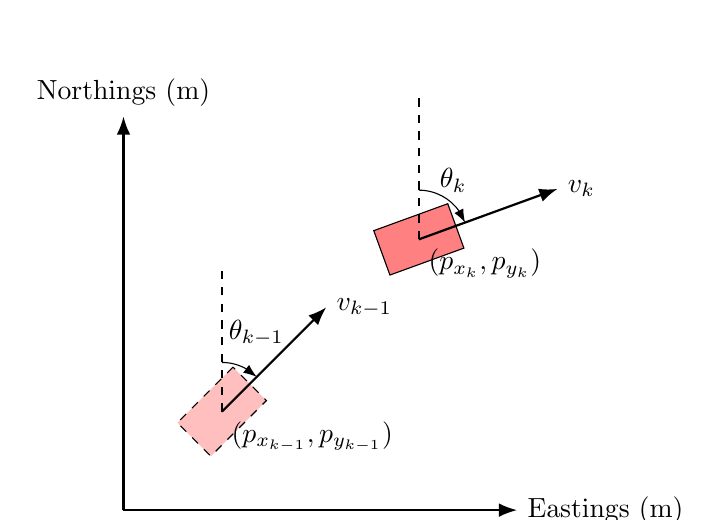
\begin{tikzpicture}[scale=1.25, >=Latex]
        % Define rotation angles
        \def\angleKminusOne{45}
        \def\angleK{20}
        
        % Draw axes
        \draw[thick,->] (0,0) -- (0,4) node[anchor=south] {Northings (m)};
        \draw[thick,->] (0,0) -- (4,0) node[anchor=west] {Eastings (m)};
        
        % Define coordinates for points
        \coordinate (O) at (0,0);
        \coordinate (pk-1) at (1,1);
        \coordinate (pk) at (3,2.75);
        

        %Pk-1
        %square
        \node[draw, rectangle, minimum width=1cm, minimum height=0.6cm, anchor=center, rotate=\angleKminusOne, fill=red!25, dashed] at (pk-1) {};

        %position label
        \node[anchor=north west] at (pk-1) {$(p_{x_{k-1}},p_{y_{k-1}})$};
        %velocity vector
        \draw[thick,->] (pk-1) -- ++(\angleKminusOne:1.5cm) node[anchor= west] {$v_{k-1}$};
        % angle
        \draw[thick,dashed] (pk-1) -- ++(0cm, 1.5cm); 
        \draw[->] (pk-1) +(90:0.5cm) arc (90:\angleKminusOne:0.5cm);
        \node at ($(pk-1)+(0.35cm, 0.8cm)$) {$\theta_{k-1}$};
        
        %Pk
        %square
        \node[draw,rectangle, minimum width=1cm, minimum height=0.6cm,anchor=center,rotate=\angleK, fill=red!50] at (pk) {};
        %position label
        \node[anchor=north west] at (pk) {$(p_{x_{k}},p_{y_{k}})$};
        %velocity vector
        \draw[thick,->] (pk) -- ++(\angleK:1.5cm) node[anchor= west] {$v_{k}$};
        % angle
        \draw[thick,dashed] (pk) -- ++(0cm, 1.5cm); 
        \draw[->] (pk) +(90:0.5cm) arc (90:\angleK:0.5cm);
        \node at ($(pk)+(0.35cm, 0.6cm)$) {$\theta_{k}$};
        
    \end{tikzpicture}
    \caption{Representation of State Vector Components in Physical Space}
    \label{tikz1}
\end{figure}

\begin{figure}[h]
    \centering
    \definecolor{WaterColor}{RGB}{1,176,241}
    \begin{tikzpicture}[scale=0.75, >=Latex]
        % Clipping path for the jar shape
        \begin{scope}
            \clip (0,0) -- (0,4) -- (4,4) -- (4,0) arc[start angle=360, end angle=180, x radius=2, y radius=0.5];
            % Drawing the water, now reaching the elliptical bottom
            \fill[WaterColor] (0,0) rectangle (4,2);
        \end{scope}
        
        % Drawing the grey rectangles
        \fill [WaterColor] (4,2) arc[start angle=0, end angle=360, x radius=2, y radius=0.5]; %top water ellipse
        \fill [WaterColor] (4,0) arc[start angle=0, end angle=360, x radius=2, y radius=0.5]; %bottom water ellipse
        \draw [WaterColor!60] (4,2) arc[start angle=0, end angle=180, x radius=2, y radius=0.5]; %back surface ellipse
        \draw [thick, dotted] (0,0) arc[start angle=180, end angle=0, x radius=2, y radius=0.5]; % Dotted top half of the elliptical base
        \fill[gray] (0.8,0) rectangle (1.2,4); % left electrode
        \fill [gray] (1.2,0) arc[start angle=0, end angle=360, x radius=0.2, y radius=0.05]; %left electrode base
        \fill [gray] (1.2,4) arc[start angle=0, end angle=360, x radius=0.2, y radius=0.05]; %left electrode cap
        \fill[gray] (2.8,0) rectangle (3.2,4); % right electrode 
        \fill [gray] (3.2,0) arc[start angle=0, end angle=360, x radius=0.2, y radius=0.05]; %left electrode base
        \fill [gray] (3.2,4) arc[start angle=0, end angle=360, x radius=0.2, y radius=0.05]; %left electrode cap
        \draw [WaterColor!60] (0,2) arc[start angle=180, end angle=360, x radius=2, y radius=0.5]; %front surface ellipse
        
        % Drawing multiple red arrows at different y positions with the new arrow style
        \foreach \y in {0.6, 2.2, 3.8} {
        % Drawing a wire, then a smaller capacitor, then another wire
        \draw[red] (1.2,\y) -- (1.8,\y) to[C, color=red] (2.2,\y) -- (2.8,\y);
        }
        % Drawing the jar with rounded corners and an elliptical bottom
        \draw [very thick, rounded corners] (0,4) -- (0,0);
        \draw [very thick] (4,0) -- (4,4);
        % Measure labels for water and air sections
        \draw[<->,thick] (4.5,0) -- (4.5,2) node[midway,fill=white,anchor=west]{$xH$};
        \draw[<->,thick] (4.5,2) -- (4.5,4) node[midway,fill=white,anchor=west]{$(1-x)H$};

        % Adding nodes for air and water
        \node at (-0.5, 3) {$\varepsilon_a$}; % Node A in the middle of the air
        \node at (-0.5, 1) {$\varepsilon_w$}; % Node B in the middle of the water
        \draw [very thick] (0,0) arc[start angle=180, end angle=360, x radius=2, y radius=0.5]; % Elliptical base

    \end{tikzpicture}
    \caption{Ideal model of Capacitive Sensor}
    \label{tikz2}
\end{figure}

\begin{figure}[h]
    \centering
    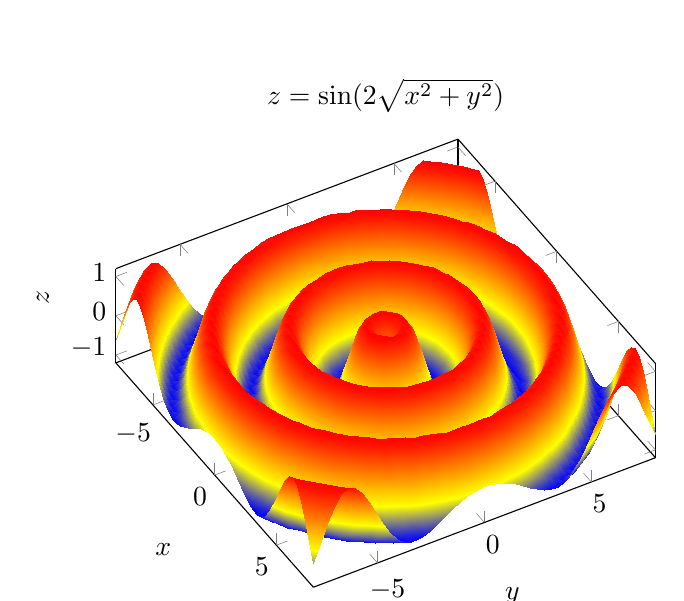
\begin{tikzpicture}
    \begin{axis}[
        title={$z = \sin(2\sqrt{x^2 + y^2})$},
        xlabel={$x$},
        ylabel={$y$},
        zlabel={$z$},
        domain=-8:8,
        y domain=-8:8,
        view={60}{70},
        samples=50
    ]
    \addplot3[
        surf,
        shader=interp,
    ]
    {sin(deg(2*sqrt(x^2 + y^2)))};
    \end{axis}
    \end{tikzpicture}
    \caption{3D plot of $z = \sin(2\sqrt{x^2 + y^2})$}
    \label{tikz3}
\end{figure}


\begin{figure}[h]
    \centering
    \begin{circuitikz}[american voltages]
        \draw
          (0,0) to [short, *-] (6,0)
          to [V, l_=$\mathrm{j}{\omega}_m \underline{\psi}^s_R$] (6,2) 
          to [R, l_=$R_R$] (6,4) 
          to [short, i_=$\underline{i}^s_R$] (5,4) 
          (0,0) to [open, v^>=$\underline{u}^s_s$] (0,4) 
          to [short, *- ,i=$\underline{i}^s_s$] (1,4) 
          to [R, l=$R_s$] (3,4)
          to [L, l=$L_{\sigma}$] (5,4) 
          to [short, i_=$\underline{i}^s_M$] (5,3) 
          to [L, l_=$L_M$] (5,0); 
        \end{circuitikz}
    
    % Caption and label for the figure
    \caption{Random Circuit I found on the internet lol} 
    \label{tikz4}
\end{figure}

circuits in particular are a major pain. If you want a circuit in your document, make it in Microcap and screenshot that (like \cref{normal_image})


\subsection{tcolorboxes}
\begin{tcolorbox}[colback=red!5!white,colframe=red!50!black,title=My nice heading]
    This is a tcolorbox with a heading. I never use tcolourboxes except for the inline code command. They're just small tcolourboxes. I thought I'd put it here anyway in case people want to use them.
\end{tcolorbox}

\begin{tcolorbox}[colback=green!5!white,colframe=green!75!black]
    Upper part of my box.
    \tcblower
    Lower part of my box. WOW!
\end{tcolorbox}


\subsection{refreencing}

You can also reference stuff. If you're doing lab reports youd be surprised how little you reference - though this does depend on the subject. If you dont want references just delete the \code{.bib} file and remove the lines in the \code{main.tex} file that have stuff to do with bibliography. That should be it I think.

Here is an example of an IEEE style reference using \code{cite()}: \cite{normal_distribution_wiki_page}



    \section{Discussion}

\note{This section will discuss the implications of the design choices, critically assessing their effectiveness and potential areas for improvement.}

The main issue will be having the interrupts not “collide” with each other since the low baud rate increases the probability that other things will interrupt the middle of a communication session with one of the SDI-12 sensors.
    \section{Conclusion}

The project successfully developed an cost-effective embedded system for monitoring and controlling environmental parameters in tropical plant research. By achieving the primary objectives, the system offers accurate data collection and environmental control, serving as a reliable alternative to expensive commercial solutions. While further refinements are needed to enhance scalability, user-friendliness, and robustness, the project provides a solid foundation for future improvements. With continued development, this system has the potential to a useful tool in environmental research applications.
    \section{Appendix}

\onecolumn
\codeblock{python}{Example Python Code}{code_example}{code/python.py}
%\codeblock{Matlab}{Example MATLAB Code}{code_example}{../code/main.m}
%if you're using the MATLAB report template

    \bibliographystyle{IEEEtranN} 
    \bibliography{references} 

\end{document}